\documentclass{ximera}

\input{../preamble.tex}

\outcome{Define accumulation functions.}
\outcome{Calculate and evaluate accumulation functions.}
\outcome{State the First Fundamental Theorem of Calculus.}
\outcome{Take derivatives of accumulation functions using the First Fundamental Theorem of Calculus.}
\outcome{Use accumulation functions to find information about the original function.}
\outcome{Understand the relationship between the function and the derivative of its accumulation function.}

\title[Dig-In:]{The First Fundamental Theorem of Calculus}

\begin{document}
\begin{abstract}
  The rate that accumulated area under a curve grows is described
  identically by that curve.
\end{abstract}
\maketitle

\section{Accumulation functions}


While the definite integral computes a signed area, which is a fixed
number, there is a way to turn it into a function.

\begin{definition}
A given a function $f$, an \dfn{accumulation function} is
\[
F(x) = \int_a^x f(t) \d t.
\]
\end{definition}
One thing that you might notice is that an accumulation function seems
to have two variables: $x$ and $t$. Let's see if we can explain
this. Consider the following graph:
\begin{image}
\begin{tikzpicture}
	\begin{axis}[
            domain=0:6, ymax=2.2,xmax=6,
            axis lines =left, xlabel=$t$, ylabel=$y$,
            width=6in,
            height=3in,
            every axis y label/.style={at=(current axis.above origin),anchor=south},
            every axis x label/.style={at=(current axis.right of origin),anchor=west},
            xtick={1,5}, ytick={.203,1.679},
            xticklabels={$a$,$x$}, yticklabels={$f(a)$,$f(x)$},
            axis on top,
          ]
          \addplot [draw=none,fill=fillp,domain=(1:5)] {sin(deg((x - 4)/2)) + 1.2} \closedcycle;
          \addplot [very thick,penColor, smooth,domain=(0:6)] {sin(deg((x - 4)/2)) + 1.2};

          \addplot [textColor,dashed] plot coordinates {(0,1.679) (5,1.679)};
          \addplot [textColor,dashed] plot coordinates {(0,.203) (1,.203)};
          %\addplot [textColor,dashed] plot coordinates {(5,0) (5,1.679)};
          \addplot [textColor] plot coordinates {(1,0) (1,.203)};

          \addplot [color=penColor,fill=penColor,only marks,mark=*] coordinates{(1,.203)};  %% closed hole         
          \addplot [color=penColor,fill=penColor,only marks,mark=*] coordinates{(5,1.679)};  %% closed hole       
          \node at (axis cs:3.4,.3) [textColor] {$F(x) = \int_a^x f(t) \d t$};
          \node at (axis cs:3.4,1) [penColor] {$f$};
        \end{axis}
\end{tikzpicture}
\end{image}

An accumulation function $F$ measures the signed area in the region
$[a,x]$ between $f$ and the $t$-axis. Hence $t$ is playing the role of
a ``place-holder'' that allows us to evaluate $f$. On the other hand,
$x$ is the \textbf{specific number} that we are using to bound the
region that will determine the area between $f$ and the $t$-axis, and
hence the value of $F$.
\begin{problem}
  Given
  \[
  F(x) = \int_{-3}^x 4 \d t,
  \]
  what is $F(5)$?
  
  \begin{prompt}
    \[
    F(5) = \answer{32}
    \]
  \end{prompt}
  \begin{problem}
    What is $F(-5)$?
    \begin{prompt}
      \[
      F(-5) = \answer{-8}
      \]
    \end{prompt}
  \end{problem}
  \end{problem}



\begin{example} 
Consider the following accumulation function for $f(x) = x^3$.
\[
F(x) = \int_{-1}^x t^3 \d t.
\]
Considering the interval $[-1,1]$, where is $F$ increasing? Where
is $F$ decreasing? When does $F$ have local extrema?

\begin{explanation}
We can see a graph of $f$ along with the signed area measured by the
accumulation function below
\begin{image}
\begin{tikzpicture}
  \begin{axis}[
      xmin=-1.2, xmax=1,ymin=-1,ymax=1,domain=-1:1,
      axis lines =center, xlabel=$t$, ylabel=$y$,
      every axis y label/.style={at=(current axis.above origin),anchor=south},
      every axis x label/.style={at=(current axis.right of origin),anchor=west},
      xtick={-1,.8}, 
      xticklabels={$-1$,$x$}, 
      axis on top,
      width=6in,
      height=3in,
    ] 
    \addplot [draw=none, fill=fillp,domain=0:.8] {x^3} \closedcycle;
    \addplot [draw=none, fill=filln,domain=-1:0] {x^3} \closedcycle;
    \addplot [penColor,very thick,domain=-1.2:1,] {x^3};
    
    \addplot [textColor] plot coordinates {(-1,0) (-1,-1)};

    \node at (axis cs:.67,.15) [textColor] {\scalebox{2}{$\boldsymbol+$}};
    \node at (axis cs:-.85,-.3) [textColor] {\scalebox{2}{$\boldsymbol-$}};
  \end{axis}
\end{tikzpicture}
%\caption{The integral $\int_{-1}^x t^3 \d t$ measures the shaded area.}
%\label{figure:accumulationeg}
\end{image}
The accumulation function starts off at zero, and then as $x$ grows,
$F$ is \wordChoice{\choice{increasing}\choice[correct]{decreasing}} as
the function accumulates negatively signed area.

However when $x>0$, $F$ starts to accumulate positively signed area,
and hence is
\wordChoice{\choice[correct]{increasing}\choice{decreasing}}. Thus $F$
is increasing on $(0,1)$, decreasing on $(-1,0)$ and hence has a local
minimum at $(0,0)$.
\end{explanation}
\end{example}

Working with the accumulation function leads us to a question, what is
\[
\int_a^x f(x) \d x
\]
when $x< a$? The general convention is that 
\[
\int_a^b f(x) \d x = -\int_b^a f(x) \d x. 
\]
With this in mind, let's consider one more example.

\begin{example} 
Consider the following accumulation function for $f(x) = x^3$.
\[
F(x) = \int_{-1}^x t^3 \d t.
\]
Where is $F$ increasing? Where is $F$ decreasing? When does
$F$ have local extrema?
\begin{explanation}
From our previous example, we know that $F$ is increasing on
$(0,1)$. Since $f$ continues to be positive at $t=1$ and beyond, $F$
is \wordChoice{\choice[correct]{increasing}\choice{decreasing}} on
$(0,\infty)$. On the other hand, we know from our previous example
that $F$ is
\wordChoice{\choice{increasing}\choice[correct]{decreasing}} on
$(-1,0)$.
\begin{image}
\begin{tikzpicture}
  \begin{axis}[
      xmin=-3, xmax=1,ymin=-10,ymax=1,domain=-3:1,
      axis lines =center, xlabel=$t$, ylabel=$y$,
      every axis y label/.style={at=(current axis.above origin),anchor=south},
      every axis x label/.style={at=(current axis.right of origin),anchor=west},
      xtick={-2,-1}, 
      xticklabels={$x$,$-1$}, 
      axis on top,
      width=6in,
      height=3in,
    ] 
    \addplot [draw=none, fill=fillp,domain=-2:-1] {x^3} \closedcycle;
    \addplot [penColor,very thick] {x^3};

    \addplot [textColor] plot coordinates {(-1,0) (-1,-1)};
    
    \node at (axis cs:-1.5,-1.5) [textColor] {\scalebox{2}{$\boldsymbol+$}};
  \end{axis}
\end{tikzpicture}
%\caption{The integral $\int_{-1}^x t^3 \d t$ measures the shaded
%  area. Note, since $x<-1$, the area has positive sign.}
\end{image}
For values to the left of $t=-1$, $F$ is still decreasing, as less and
less positively signed area is accumulated. Hence $F$ is increasing on
$(0,\infty)$, decreasing on $(-\infty,0)$ and hence has an absolute
minimum at $(0,0)$.
\end{explanation}
\end{example}
The key point to take from these examples is that an accumulation
function
\[
F(x) = \int_a^x f(t) \d t
\]
is increasing precisely when $f$ is positive and is decreasing
precisely when $f$ is negative. In short, it seems that $f$ is
behaving in a similar fashion to $F'$.



\section{The First Fundamental Theorem of Calculus}



Let $f$ be a continuous function on the real numbers and consider
\[
  F(x) = \int_a^x f(t)\d t.
\]
From our previous work we know that $F$ is increasing when $f$ is
positive and $F$ is decreasing when $f$ is negative. Moreover, with
careful observation, we can even see that $F$ is concave up when $f'$
is positive and that $F$ is concave down when $f'$ is negative.
Thinking about what we have learned about the relationship of a
function to its first and second derivatives, it is not too hard to
guess that there must be a connection between $F'$ and the function
$f$. This is a good guess, check out our next theorem:


\begin{theorem}[First Fundamental Theorem of Calculus]\index{First Fundamental Theorem of Calculus}
Suppose that $f$ is continuous on the real numbers and let
\[
  F(x)=\int_a^x f(t)\d t.
\]
Then $F'(x)=f(x)$.
\end{theorem}
The First Fundamental Theorem of Calculus says that an accumulation
function of $f$ is an antiderivative of $f$. Another way of saying
this is:
\begin{image}
  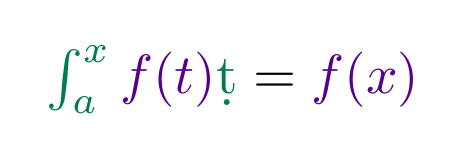
\begin{tikzpicture}[scale=2,every node/.style={transform shape}]
    \node at (0,0) {
      $\color{blue!70!green}\ddx \color{green!70!black!70!blue}\int_a^x\color{purple!50!blue!90!black}f(t)\color{green!70!black!70!blue}\d t\color{black} = \color{purple!50!blue!90!black}f(x)$
      };
  \end{tikzpicture}
\end{image}
This could be read as:%%BADBAD I want this all in bold and with colors
\begin{quote}\large\textbf{The \textcolor{blue!70!green}{rate} that \textcolor{green!70!black!70!blue}{accumulated area} under a  \textcolor{purple!50!blue!90!black}{curve} grows is described identically by that  \color{purple!50!blue!90!black}{curve}.}
\end{quote}

Now that we are working with accumulation functions, let's see what
happens when we compose them with other functions.

\begin{example}
  Find the derivative of
  \[
  F(x) = \int_2^{x^2} \cos t \d t.
  \]
  \begin{explanation}
    Consider 
    \[
    G(x) = \int_2^x \cos t \d t
    \]
    and set $h(x) = \answer[given]{x^2}$. Now
    \[
    F(x) = G(h(x)).
    \]
    The First Fundamental Theorem of Calculus states that $G'(x) = \cos x$. The chain rule gives us
    \begin{align*}
      F'(x) &= G'(h(x)) h'(x) \\
      &= \cos (h(x)) h'(x) \\
      &= \answer[given]{\cos (x^2) 2x}.
    \end{align*}
  \end{explanation}
\end{example}

Let's practice this once more.

\begin{example}
  Find the
  derivative of
  \[
  F(x) = \int_{\cos x}^5 t^3\d t.
  \]
  \begin{explanation}
    Consider
    \[
    G(x) = - \int_5^x t^3 \d t
    \]
    and set $h(x) = \answer[given]{\cos(x)}$. Now
    \[
    F(x) = G(h(x)).
    \]
    The First Fundamental Theorem of Calculus states that $G'(x) = -x^3$. The chain rule gives us
    \begin{align*}
      F'(x) &= G'(h(x))h'(x)\\
      &=-h(x)^3 h'(x)\\
      &=\answer[given]{-\cos^3(x) (-\sin(x))}.
    \end{align*}
  \end{explanation}
\end{example}


















\end{document}
